\newpage

\section{Problem 5.27}

此题采用线搜索确定步长时,得到的结果误差极大,因为$\phi'(0)$在离稳定点较远时数量级高达$10^{40}$量级,导致线搜索得到的步长极小,几乎为0,无法收敛,经反复调整参数都没能取得好的结果,最后只好手动确定步长$\alpha_k=0.05$,此时效果良好,残量的2-范数随迭代次数的下降情况如下:(由于数量级巨大,为了更好的显示残差的波动,将原图中将残差取对数处理后并排参考)

\begin{figure}[H]
\centering
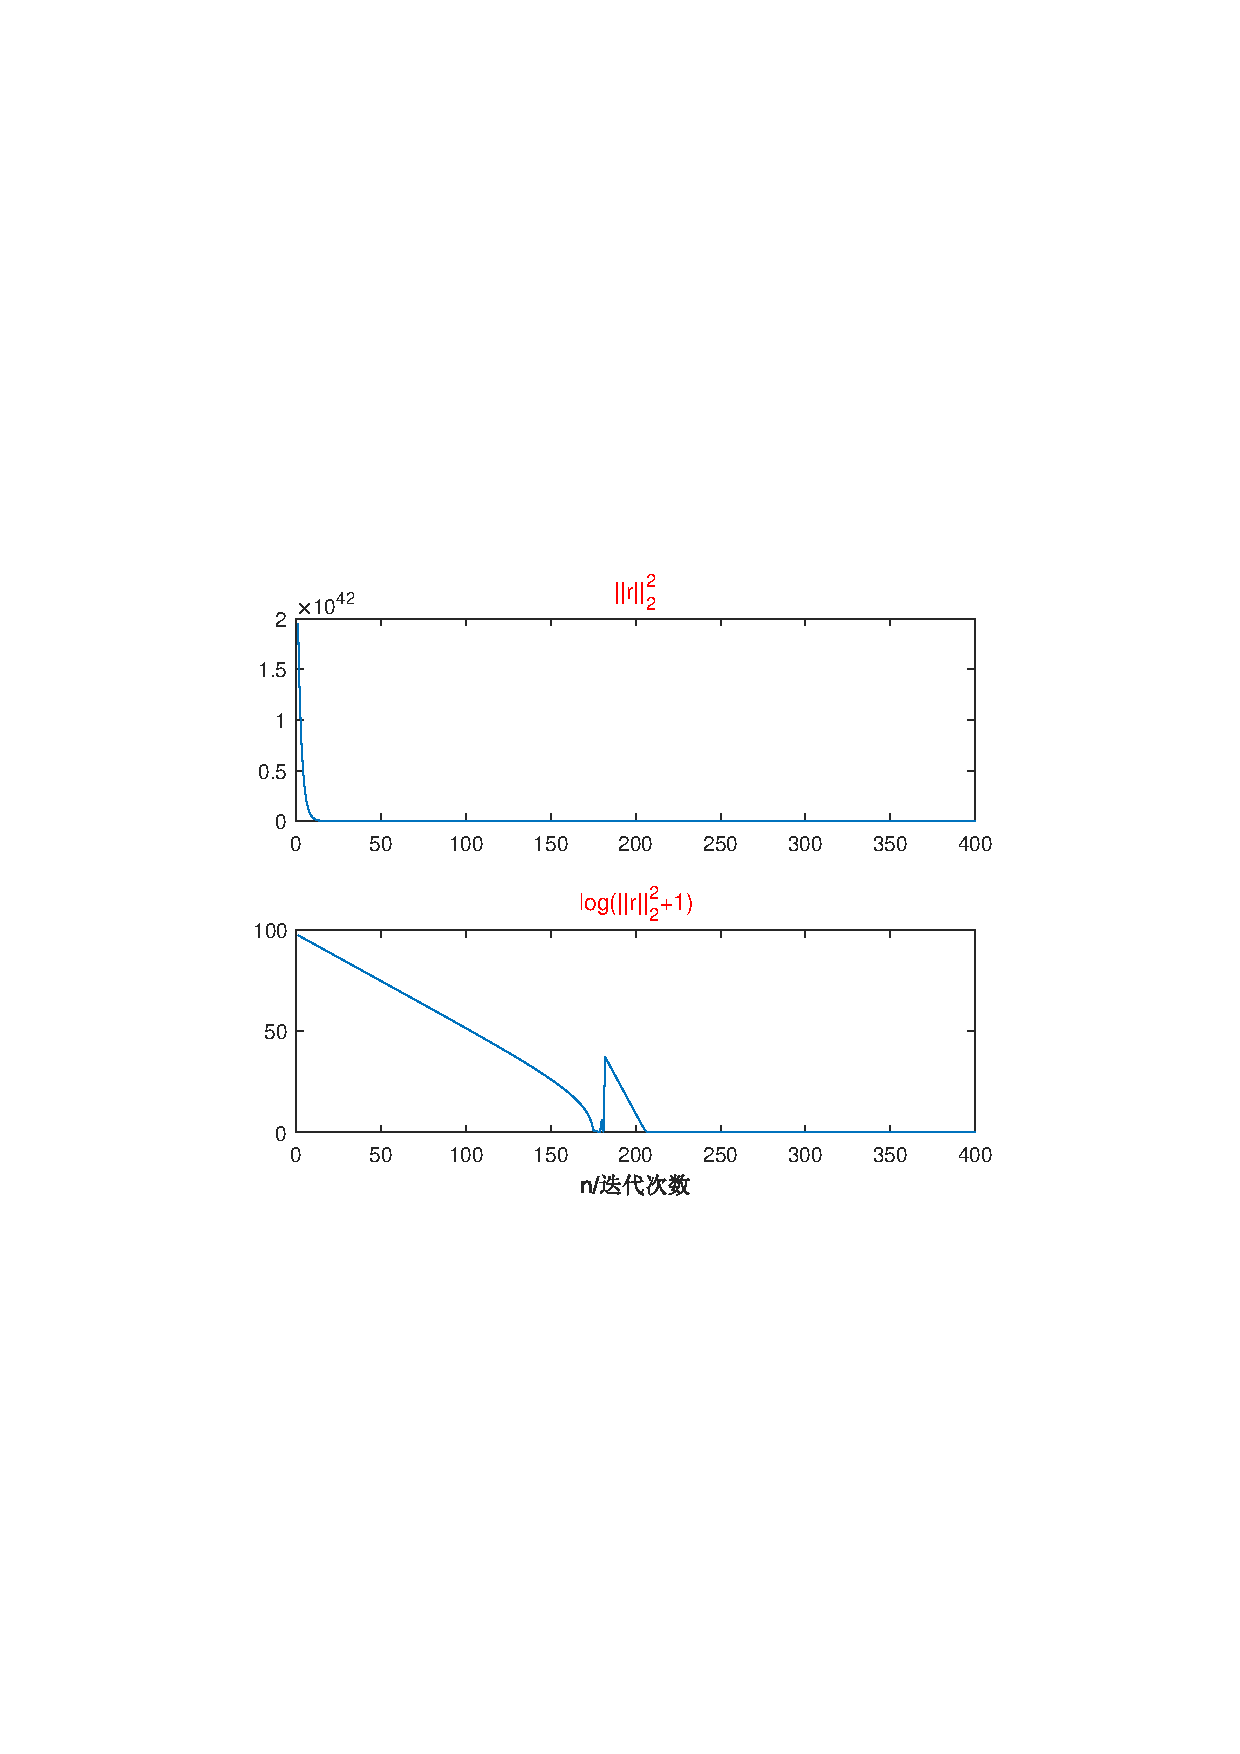
\includegraphics[width=12cm]{fig/6_1.pdf}
\end{figure}



又采用MATLAB中优化工具箱中的lsqnonlin函数进行拟合,得到的结果比我的程序算出来的略好,将两者进行比较,比较结果如下:

\begin{figure}[H]
\centering
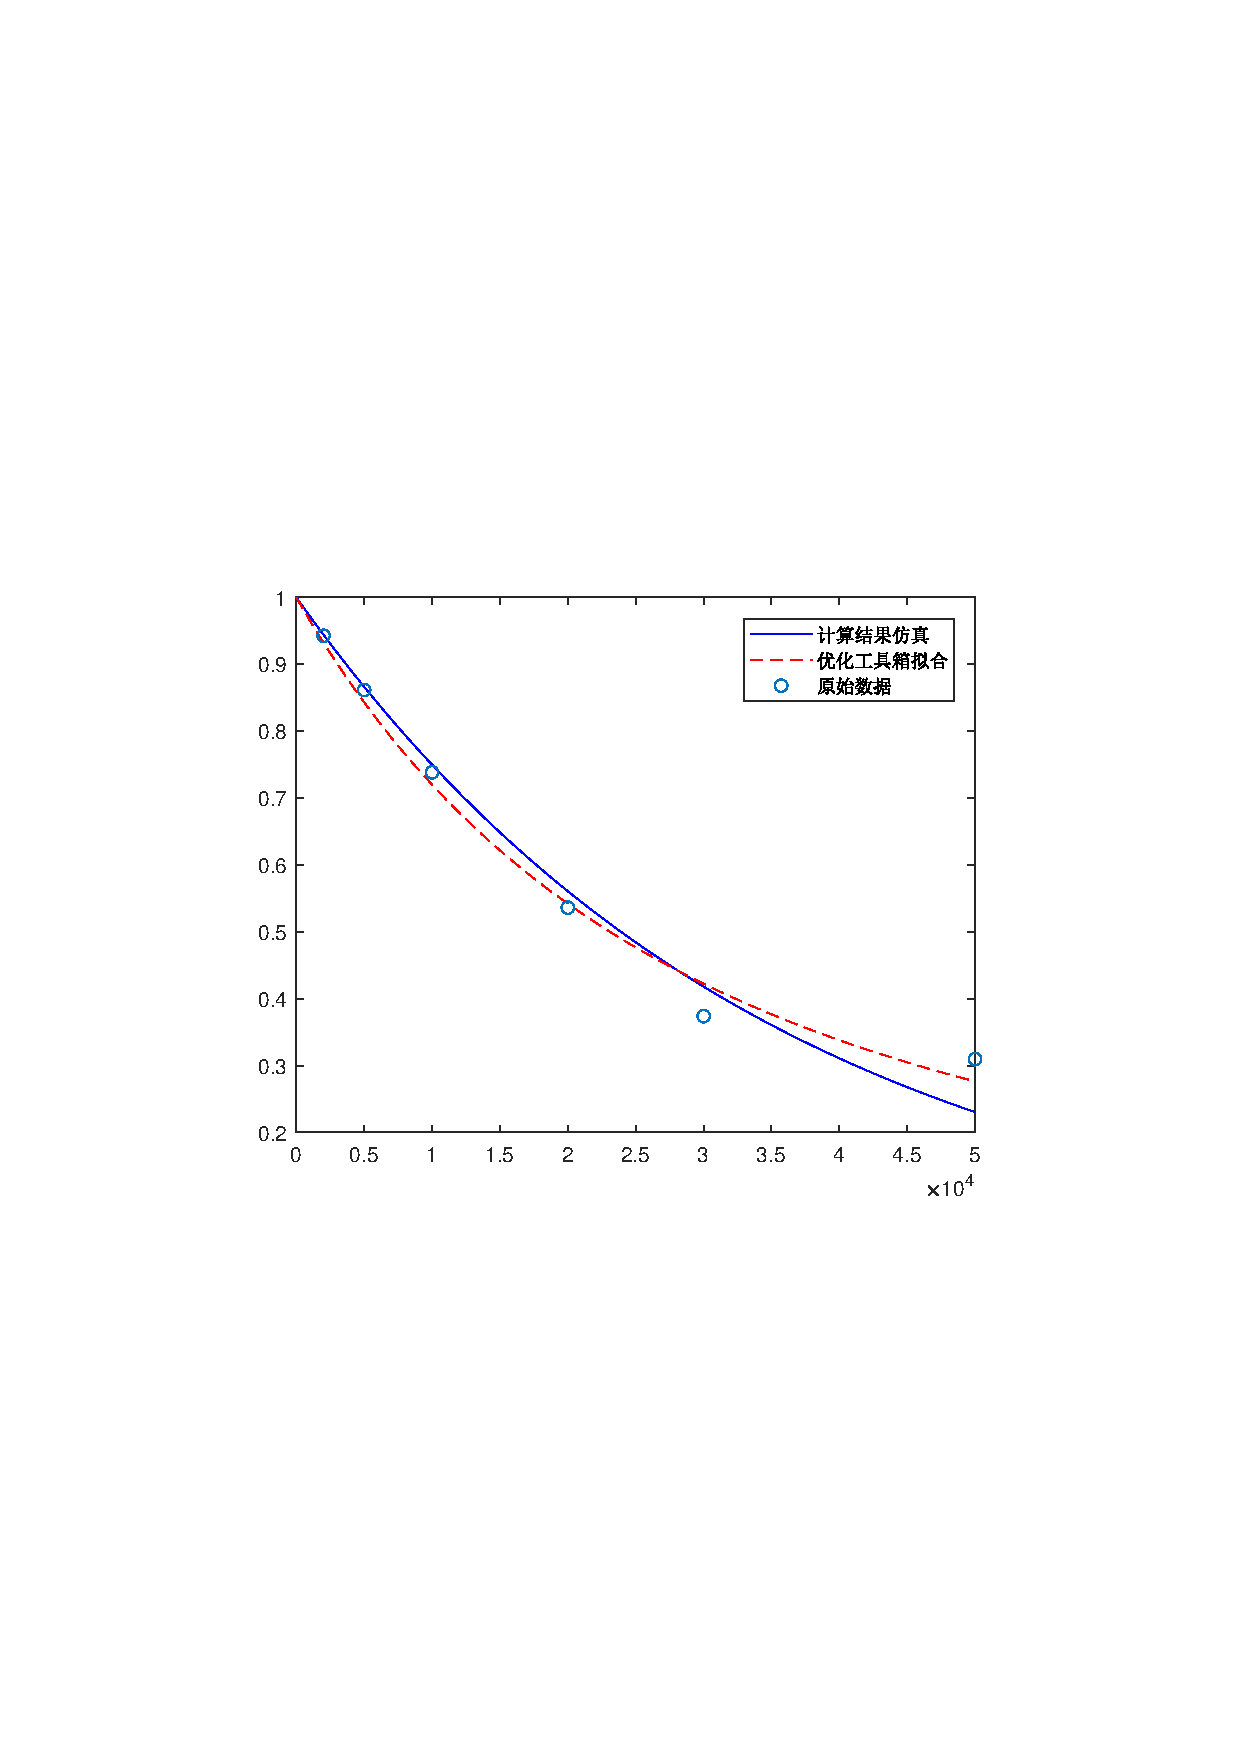
\includegraphics[width=12cm]{fig/6_2.pdf}
\end{figure}

\subsection{计算结果展示}
\begin{table}[H]
\centering
\caption{结果比较}
	\begin{tabular}{ccc}
	\toprule
	{}&程序计算&工具箱拟合\\
	\midrule
	stv&0.125639950119876&0.104420208306470\\
	$x_1$&3.323336983976929e-04&-0.009615612533368\\
	$x_2$&3.516673367231929e+02&-19.446505801429495\\
	\bottomrule
	\end{tabular}
\end{table}


\subsection{算法伪代码}
\begin{algorithm}[h]  
\caption{Gauss-Newton method for problem(5.27)}  
\begin{algorithmic}[1]  
\STATE Given $\bm{x}^{(0)}$ and $G$
\STATE Set $\bm{p}^{(0)}=-\bm{g}^{(0)},k=0$
\WHILE {$\|\bm{g}^{(k)}\|>\epsilon$}
\STATE Set $\alpha_k=-\dfrac{{{\bm{p}^{(k)}}^T}\bm{g}^{(k)}}{{\bm{p}^{(k)}}^T\bm{G}\bm{p}^{(k)}}$
\STATE Set $\bm{x}^{(k+1)}=\bm{x}^{(k)}+\alpha_k\bm{p}^{(k)}$
\STATE Set $\bm{g}^{(k+1)}=g(\bm{x}^{(k+1)})$
\STATE Set $\bm{p}^{(k)}=-\bm{g}^{(k)}$
\STATE k=k+1
\ENDWHILE
\end{algorithmic}  
\end{algorithm}  

